\documentclass[11pt]{article}

\usepackage[margin=1in]{geometry}
\usepackage[T1]{fontenc}
\usepackage{lmodern}
\usepackage{microtype}
\usepackage{amsmath,amssymb,amsthm,mathtools}
\usepackage{mathrsfs}
\usepackage[dvipsnames]{xcolor}
\usepackage[most]{tcolorbox}
\usepackage{tikz}
\usetikzlibrary{decorations.markings,patterns}
\usepackage{enumitem}
\usepackage{tocloft}
\usepackage[hidelinks]{hyperref}

\definecolor{courseblue}{HTML}{1F4E79}
\definecolor{lightblue}{HTML}{EAF2F8}
\definecolor{lightgreen}{HTML}{EAF7EA}
\definecolor{lightpink}{HTML}{FCE8EF}
\definecolor{lightyellow}{HTML}{FFF8D6}
\definecolor{warningyellow}{HTML}{D6A000}
\definecolor{exercisebg}{HTML}{FDEAEA}
\definecolor{exerciseframe}{HTML}{B54040}
\definecolor{examplebg}{HTML}{F4FAFE}
\definecolor{exampleframe}{HTML}{85C1E9}
\definecolor{darkgray}{HTML}{333333}
\definecolor{lightorange}{HTML}{FDEBD8}
\definecolor{orangeframe}{HTML}{E08A3C}
\definecolor{remarkbg}{HTML}{F3EEFB}
\definecolor{remarkframe}{HTML}{9B7FC9}

\setlength{\parindent}{0pt}
\setlength{\parskip}{0.45em}
\setlist[itemize]{topsep=0.25em,itemsep=0.15em}
\renewcommand{\cftsecleader}{\cftdotfill{\cftdotsep}}
\renewcommand{\cftsubsecleader}{\cftdotfill{\cftdotsep}}

\theoremstyle{plain}
\newtheorem{theorem}{Theorem}[section]
\newtheorem{proposition}[theorem]{Proposition}
\newtheorem{lemma}[theorem]{Lemma}
\newtheorem{corollary}[theorem]{Corollary}
\theoremstyle{definition}
\newtheorem{definition}[theorem]{Definition}
\newtheorem{example}[theorem]{Example}
\newtheorem{exercise}[theorem]{Exercise}
\theoremstyle{remark}
\newtheorem*{remark}{Remark}
\newtheorem*{fact}{Fact}
\newtheorem*{warning}{Warning}

\tcolorboxenvironment{definition}{
  enhanced,
  unbreakable,
  colback=lightgreen,
  colframe=ForestGreen,
  boxrule=0.7pt,
  arc=2pt,
  left=6pt,
  right=6pt,
  top=5pt,
  bottom=5pt
}

\tcolorboxenvironment{remark}{
  enhanced,
  colback=remarkbg,
  colframe=remarkframe,
  before upper={\setlength{\parskip}{0.5em}},
  boxrule=0.7pt,
  arc=2pt,
  left=6pt,
  right=6pt,
  top=5pt,
  bottom=5pt
}

\tcolorboxenvironment{warning}{
  enhanced,
  colback=lightyellow,
  colframe=warningyellow,
  boxrule=0.7pt,
  arc=2pt,
  left=6pt,
  right=6pt,
  top=5pt,
  bottom=5pt
}

\tcolorboxenvironment{exercise}{
  enhanced,
  colback=exercisebg,
  colframe=exerciseframe,
  boxrule=1pt,
  arc=2pt,
  left=6pt,
  right=6pt,
  top=5pt,
  bottom=5pt
}

\tcolorboxenvironment{example}{
  enhanced,
  colback=examplebg,
  colframe=exampleframe,
  boxrule=0.7pt,
  arc=2pt,
  left=6pt,
  right=6pt,
  top=5pt,
  bottom=5pt
}

\numberwithin{equation}{section}

\newcommand{\be}{\begin{eqnarray}}
\newcommand{\ee}{\end{eqnarray}}
\newcommand{\C}{\mathbb{C}}
\newcommand{\R}{\mathbb{R}}
\newcommand{\N}{\mathbb{N}}
\newcommand{\Z}{\mathbb{Z}}
\DeclareMathOperator{\Log}{Log}
\DeclareMathOperator{\Arg}{Arg}

\DeclareMathOperator{\Hol}{\mathcal{H}\mathrm{ol}}
\DeclareMathOperator{\Real}{Re}
\DeclareMathOperator{\Imag}{Im}
\newcommand{\A}{\mathcal{A}}
\newcommand{\CT}{\C[[T]]}
\newcommand{\CLT}{\C((T))}
\tcbset{breakable}
% Compact spacing around diagrams; keep the main text at 11pt.
\newenvironment{lecturefigure}
 {\par\addvspace{0.25em}\begingroup\setlength{\parskip}{0pt}\centering}
 {\par\endgroup\addvspace{0.25em}}
\begin{document}

\begin{center}
  \colorbox{lightblue}{%
    \begin{minipage}{0.94\textwidth}
      \vspace{0.55em}
      \begin{tabular*}{\textwidth}{@{\extracolsep{\fill}}lr}
        {\color{courseblue}\bfseries\LARGE Lecture 23} &
        {\color{courseblue}\bfseries\LARGE MATH 411}\\[0.35em]
        \textbf{Fall 2026} & \textbf{Date: Nov 2, 2026}\\
        & \textbf{Instructor: Manish Patnaik}
      \end{tabular*}
      \vspace{0.45em}
    \end{minipage}}
\end{center}

\setcounter{tocdepth}{1}
\tableofcontents
\vspace{0.45em}

% Sources: handwritten Lecture 23, Nov. 4, pages 1--8. Order follows the
% handwritten notes: winding numbers, the residue theorem and its proof,
% tricks for computing residues, a square-contour example, trigonometric
% integrals, improper integrals. Added: the null-homotopy hypothesis in the
% residue theorem, a proof that winding numbers are integers, and the
% completed computations of the two examples left open on pages 6 and 8.
In Lecture~22 we expanded a function with an isolated singularity in a
Laurent series. Today we use the coefficient $a_{-1}$ of that series, the
\emph{residue}, to evaluate contour integrals around several singularities
at once. We then apply the resulting residue theorem to compute real
integrals.

\section{Winding numbers and residues}
% Handwritten Lecture 23, page 1.
\subsection{Winding numbers}
Let $\gamma\colon[a,b]\to\C$ be a closed piecewise $C^1$ curve and let
$\alpha\in\C$ be a point not on $\gamma$. Intuitively, the \emph{winding
number} $w(\gamma,\alpha)$ is the number of times $\gamma$ wraps around
$\alpha$ in the counterclockwise direction. Analytically:

\begin{definition}
The \emph{winding number} of $\gamma$ around $\alpha$ is
\[
 w(\gamma,\alpha)=\frac{1}{2\pi i}\int_\gamma\frac{dz}{z-\alpha}.
\]
\end{definition}
In Lecture~22 we wrote $n(\gamma,\alpha)$ for the same quantity. For the
circle $C(t)=\alpha+\rho e^{it}$, $0\leq t\leq2\pi$, we have
$w(C,\alpha)=1$; going around $k$ times, $t\in[0,2\pi k]$, gives $k$.

\begin{proposition}\label{prop:winding-integer}
$w(\gamma,\alpha)$ is an integer.
\end{proposition}
\begin{proof}
Put $h(t)=\int_a^t\frac{\gamma'(s)}{\gamma(s)-\alpha}\,ds$, so that
$h(b)=2\pi i\,w(\gamma,\alpha)$. Away from the finitely many corners,
\[
 \frac{d}{dt}\Bigl[(\gamma(t)-\alpha)e^{-h(t)}\Bigr]
 =\gamma'(t)e^{-h(t)}-(\gamma(t)-\alpha)\frac{\gamma'(t)}{\gamma(t)-\alpha}e^{-h(t)}=0.
\]
The bracket is continuous, so it is constant on $[a,b]$. Comparing $t=a$
and $t=b$ and using $\gamma(a)=\gamma(b)$ gives $e^{-h(b)}=1$, so
$h(b)\in2\pi i\Z$.
\end{proof}

\begin{lecturefigure}
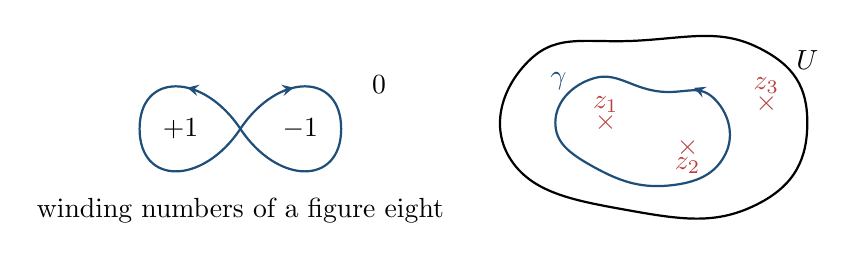
\begin{tikzpicture}[scale=0.8,>=stealth]
 \begin{scope}
  \draw[courseblue,thick,postaction={decorate},decoration={markings,
   mark=at position 0.12 with {\arrow{>}},mark=at position 0.62 with {\arrow{>}}}]
   (0,0) .. controls (0.6,0.9) and (1.6,0.9) .. (1.6,0)
         .. controls (1.6,-0.9) and (0.6,-0.9) .. (0,0)
         .. controls (-0.6,0.9) and (-1.6,0.9) .. (-1.6,0)
         .. controls (-1.6,-0.9) and (-0.6,-0.9) .. (0,0);
  \node at (-0.95,0) {$+1$};
  \node at (0.95,0) {$-1$};
  \node at (2.2,0.7) {$0$};
  \node[below] at (0,-0.95) {winding numbers of a figure eight};
 \end{scope}
 \begin{scope}[xshift=6.6cm]
  \draw[thick] plot[smooth cycle,tension=0.8] coordinates
   {(-2.3,-0.5) (-2,1.1) (-0.3,1.4) (1.6,1.3) (2.4,0.1)
    (1.6,-1.2) (-0.4,-1.3)};
  \node at (2.4,1.1) {$U$};
  \draw[courseblue,thick,postaction={decorate},decoration={markings,
   mark=at position 0.25 with {\arrow{<}}}]
   plot[smooth cycle,tension=0.8] coordinates
   {(-1.6,0.1) (-1,0.8) (0,0.6) (0.9,0.5) (1.1,-0.4) (0.2,-0.9) (-1,-0.6)};
  \node[exerciseframe] at (-0.8,0.1) {$\times$};
  \node[exerciseframe,above] at (-0.8,0.1) {$z_1$};
  \node[exerciseframe] at (0.5,-0.3) {$\times$};
  \node[exerciseframe,below] at (0.5,-0.3) {$z_2$};
  \node[exerciseframe] at (1.75,0.4) {$\times$};
  \node[exerciseframe,above] at (1.75,0.4) {$z_3$};
  \node[courseblue] at (-1.55,0.75) {$\gamma$};
 \end{scope}
\end{tikzpicture}

{\small Left: $w=+1$ in the left lobe, $-1$ in the right lobe, $0$ outside. Right:
$w(\gamma,z_1)=w(\gamma,z_2)=1$, $w(\gamma,z_3)=0$.}
\end{lecturefigure}

\subsection{Residues}
\begin{definition}
Suppose $f$ has an isolated singularity at $z_0$, with Laurent expansion
$f(z)=\sum_{n\in\Z}a_n(z-z_0)^n$ on $0<|z-z_0|<\rho$. The \emph{residue}
of $f$ at $z_0$ is
\[
 \operatorname{Res}_{z_0}(f)=a_{-1}
 =\frac{1}{2\pi i}\int_{|z-z_0|=r}f(z)\,dz\qquad(0<r<\rho).
\]
The \emph{principal part} of $f$ at $z_0$ is
$f_-(z)=\sum_{n<0}a_n(z-z_0)^n$.
\end{definition}
The integral formula is the coefficient formula of Lecture~21 with
$n=-1$. The principal part is a power series in $1/(z-z_0)$ with infinite
radius of convergence (it converges for every $z\ne z_0$), so $f_-$ is
holomorphic on $\C\setminus\{z_0\}$.

\section{The residue theorem}
% Handwritten Lecture 23, pages 1--2.
\begin{theorem}[Residue theorem]\label{thm:residue}
Let $U\subseteq\C$ be open, let $z_1,\dots,z_n\in U$ be distinct, and let
$f$ be holomorphic on $U\setminus\{z_1,\dots,z_n\}$. Let $\gamma$ be a closed
piecewise $C^1$ curve in $U\setminus\{z_1,\dots,z_n\}$ that is
null-homotopic in $U$ (for instance, any such curve when $U$ is simply
connected). Then
\[
 \boxed{\displaystyle\int_\gamma f(z)\,dz
 =2\pi i\sum_{j=1}^{n}w(\gamma,z_j)\operatorname{Res}_{z_j}(f).}
\]
\end{theorem}

\begin{warning}
Some hypothesis on $\gamma$ relative to $U$ is needed. On
$U=\C\setminus\{0\}$ the function $f(z)=1/z$ has no singularities at all,
yet $\int_{|z|=1}dz/z=2\pi i$. The unit circle is not null-homotopic in $U$.
\end{warning}

\begin{proof}
Let $f_-^{(j)}$ be the principal part of $f$ at $z_j$, so near $z_j$
\[
 f(z)=f_-^{(j)}(z)+f_+^{(j)}(z),
\]
where $f_-^{(j)}$ involves only negative powers of $z-z_j$ and $f_+^{(j)}$
is a power series, holomorphic near $z_j$. Define
\[
 g(z)=f(z)-\sum_{j=1}^{n}f_-^{(j)}(z),
\]
that is, subtract the principal parts at $z_1,\dots,z_n$.

\textbf{Claim: $g$ extends to a holomorphic function on $U$.} Each
$f_-^{(k)}$ is holomorphic on $\C\setminus\{z_k\}$, so $g$ is holomorphic on
$U\setminus\{z_1,\dots,z_n\}$. Near $z_j$,
\[
 g=f_+^{(j)}-\sum_{k\ne j}f_-^{(k)},
\]
which is holomorphic at $z_j$. So the singularity of $g$ at each $z_j$ is
removable, and $g$ extends.

By the null-homotopy corollary of Lecture~18, $\int_\gamma g=0$, that is,
\[
 \int_\gamma f=\sum_{j=1}^{n}\int_\gamma f_-^{(j)}.
\]
Now write
\[
 f_-^{(j)}(z)=\frac{a_{-1}^{(j)}}{z-z_j}+\frac{a_{-2}^{(j)}}{(z-z_j)^2}+\cdots.
\]
Since $\gamma$ stays a positive distance $\delta$ from $z_j$, the series
converges uniformly on $\gamma$ (it is a power series in $1/(z-z_j)$, and
$|1/(z-z_j)|\leq1/\delta$ there). We may therefore integrate term by term
(Lecture~20, Corollary~2.2). For $k\geq2$, $(z-z_j)^{-k}$ has the primitive
$(z-z_j)^{1-k}/(1-k)$ on $\C\setminus\{z_j\}$, so its integral over the
closed curve $\gamma$ vanishes. Only the first term survives:
\[
 \int_\gamma f_-^{(j)}
 =\underbrace{a_{-1}^{(j)}}_{\operatorname{Res}_{z_j}(f)}
 \underbrace{\int_\gamma\frac{dz}{z-z_j}}_{2\pi i\,w(\gamma,z_j)}.
\]
Summing over $j$ proves the theorem.
\end{proof}

In the most common situation, $\gamma$ is a simple closed curve traversed
counterclockwise; then $w(\gamma,z_j)$ is $1$ for the singularities inside
$\gamma$ and $0$ for those outside, and $\int_\gamma f$ is $2\pi i$ times the
sum of the residues inside.

\section{Computing residues}
% Handwritten Lecture 23, pages 3--4.
A pole of order $1$ is called a \emph{simple pole}. Two tricks handle most
simple poles.

\begin{proposition}\label{prop:res-product}
If $f$ has a simple pole at $z_0$ and $g$ is holomorphic at $z_0$, then
\[
 \operatorname{Res}_{z_0}(fg)=g(z_0)\operatorname{Res}_{z_0}(f).
\]
\end{proposition}
\begin{proof}
Write $f=\frac{a_{-1}}{z-z_0}+a_0+a_1(z-z_0)+\cdots$ and
$g=b_0+b_1(z-z_0)+\cdots$ with $b_0=g(z_0)$. Multiplying,
\[
 fg=\frac{a_{-1}b_0}{z-z_0}+(\text{power series in }z-z_0),
\]
so $\operatorname{Res}_{z_0}(fg)=a_{-1}b_0=g(z_0)\operatorname{Res}_{z_0}(f)$.
\end{proof}

\begin{proposition}\label{prop:res-simple-zero}
Let $f$ be holomorphic near $z_0$ with $f(z_0)=0$ and $f'(z_0)\ne0$. Then
$1/f$ has a simple pole at $z_0$, and
\[
 \operatorname{Res}_{z_0}\Bigl(\frac1f\Bigr)=\frac{1}{f'(z_0)}.
\]
\end{proposition}
\begin{proof}
Expand $f(z)=a_0+a_1(z-z_0)+a_2(z-z_0)^2+\cdots$, where $a_0=f(z_0)=0$ and
$a_1=f'(z_0)\ne0$. Then
\[
 f(z)=a_1(z-z_0)\,h(z),\qquad
 h(z)=1+\frac{a_2}{a_1}(z-z_0)+\cdots,
\]
and $h$ is holomorphic at $z_0$ with $h(z_0)=1$, hence nonzero near $z_0$.
So $1/h$ is holomorphic near $z_0$ with $1/h=1+b_1(z-z_0)+\cdots$, and
\[
 \frac1f=\frac{1}{a_1}\cdot\frac{1}{z-z_0}\cdot\frac1h
 =\frac{1}{a_1}\,\frac{1}{z-z_0}+(\text{power series in }z-z_0).
\]
Thus the pole is simple with residue $1/a_1=1/f'(z_0)$.
\end{proof}
Combining the two propositions: if $g$ is holomorphic at $z_0$, $f(z_0)=0$
and $f'(z_0)\ne0$, then
$\operatorname{Res}_{z_0}(g/f)=g(z_0)/f'(z_0)$.

\begin{example}[A square contour]
% Handwritten page 4 writes z_1 = 1 + i\sqrt2; the roots are -1 \pm i\sqrt2.
Let $p(z)=z^2+2z+3=(z-z_1)(z-z_2)$ with
\[
 z_1=-1+i\sqrt2,\qquad z_2=-1-i\sqrt2,
\]
and let $C$ be the boundary of the square centred at $0$ with side
length $8$, traversed counterclockwise. Both roots lie inside $C$, so
$w(C,z_1)=w(C,z_2)=1$ and, by Proposition~\ref{prop:res-simple-zero} with
$p'(z)=2z+2$,
\[
 \int_C\frac{dz}{p(z)}
 =2\pi i\left(\frac{1}{p'(z_1)}+\frac{1}{p'(z_2)}\right)
 =2\pi i\left(\frac{1}{2i\sqrt2}-\frac{1}{2i\sqrt2}\right)=0.
\]
\begin{lecturefigure}
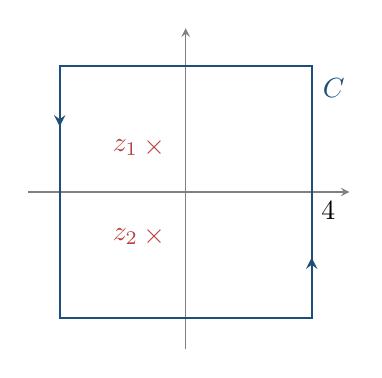
\begin{tikzpicture}[scale=0.4,>=stealth]
 \draw[gray,->] (-5,0)--(5.2,0);
 \draw[gray,->] (0,-5)--(0,5.2);
 \draw[courseblue,thick,postaction={decorate},decoration={markings,
  mark=at position 0.06 with {\arrow{>}},mark=at position 0.56 with {\arrow{>}}}]
  (4,-4)--(4,4)--(-4,4)--(-4,-4)--cycle;
 \node[exerciseframe] at (-1,1.414) {$\times$};
 \node[exerciseframe] at (-1,-1.414) {$\times$};
 \node[exerciseframe,left] at (-1.2,1.414) {$z_1$};
 \node[exerciseframe,left] at (-1.2,-1.414) {$z_2$};
 \node[below right] at (4,0) {$4$};
 \node[courseblue] at (4.7,3.3) {$C$};
\end{tikzpicture}
\end{lecturefigure}
\end{example}

\begin{exercise}
Show that if $f$ has a pole of order $m$ at $z_0$, then
\[
 \operatorname{Res}_{z_0}(f)=\frac{1}{(m-1)!}\lim_{z\to z_0}
 \frac{d^{m-1}}{dz^{m-1}}\Bigl[(z-z_0)^mf(z)\Bigr].
\]
Use it to compute $\operatorname{Res}_0\bigl(e^z/z^3\bigr)$, and check your
answer against the Laurent series.
\end{exercise}

\section{Trigonometric integrals}
% Handwritten Lecture 23, pages 5--6. The handwritten substitution uses
% \bar z; on the unit circle \bar z = 1/z, which is what makes the
% integrand holomorphic. The example on page 6 is completed here.
Let $Q(x,y)=P(x,y)/R(x,y)$ be a rational function of two real variables
($P,R$ polynomials), and suppose $R(\cos\theta,\sin\theta)\ne0$ for all
$\theta$. An integral of the form
\[
 \int_0^{2\pi}Q(\cos\theta,\sin\theta)\,d\theta
\]
is called a \emph{trigonometric integral}. For example,
\[
 \int_0^{2\pi}\frac{\cos^2\theta-\sin^2\theta+\cos\theta\sin\theta}
 {3-\sin\theta}\,d\theta
 \qquad\text{has}\qquad
 Q(x,y)=\frac{x^2-y^2+xy}{3-y}.
\]

On the unit circle $z=e^{i\theta}=\cos\theta+i\sin\theta$ we have
$\bar z=e^{-i\theta}=1/z$, so
\[
 \cos\theta=\frac{z+\bar z}{2}=\frac12\Bigl(z+\frac1z\Bigr),\qquad
 \sin\theta=\frac{z-\bar z}{2i}=\frac{1}{2i}\Bigl(z-\frac1z\Bigr).
\]
Parametrizing the unit circle $C$ by $\gamma(\theta)=e^{i\theta}$, with
$\gamma'(\theta)=ie^{i\theta}$, we get
\[
 \int_C Q\Bigl(\tfrac12\bigl(z+\tfrac1z\bigr),\tfrac1{2i}\bigl(z-\tfrac1z\bigr)\Bigr)
 \frac{dz}{iz}
 =\int_0^{2\pi}Q(\cos\theta,\sin\theta)\,\frac{ie^{i\theta}}{ie^{i\theta}}\,d\theta
 =\int_0^{2\pi}Q(\cos\theta,\sin\theta)\,d\theta.
\]
Writing $1/z$ rather than $\bar z$ is essential: the integrand on the left
is then a rational function of $z$, and the residue theorem applies to it
on the disc $|z|<1+\epsilon$.

\begin{example}
Let $a>1$ be real. We compute $\displaystyle\int_0^{2\pi}\frac{d\theta}{a+\sin\theta}$.
Here $Q(x,y)=1/(a+y)$, and
\[
 \frac{1}{a+\frac{1}{2i}(z-\frac1z)}\cdot\frac{1}{iz}
 =\frac{2iz}{z^2+2iaz-1}\cdot\frac{1}{iz}
 =\frac{2}{z^2+2iaz-1}.
\]
The roots of $z^2+2iaz-1$ are
\[
 z_\pm=i\bigl(-a\pm\sqrt{a^2-1}\bigr).
\]
Since $z_+z_-=-1$ and $|z_-|=a+\sqrt{a^2-1}>1$, only $z_+$ lies inside the
unit circle. By Proposition~\ref{prop:res-simple-zero},
\[
 \operatorname{Res}_{z_+}\frac{2}{z^2+2iaz-1}=\frac{2}{2z_++2ia}
 =\frac{1}{i\sqrt{a^2-1}}.
\]
Therefore
\[
 \boxed{\int_0^{2\pi}\frac{d\theta}{a+\sin\theta}
 =2\pi i\cdot\frac{1}{i\sqrt{a^2-1}}=\frac{2\pi}{\sqrt{a^2-1}}\qquad(a>1).}
\]
As a check, for large $a$ the integrand is close to $1/a$ and the answer
is close to $2\pi/a$.
\end{example}

\begin{lecturefigure}
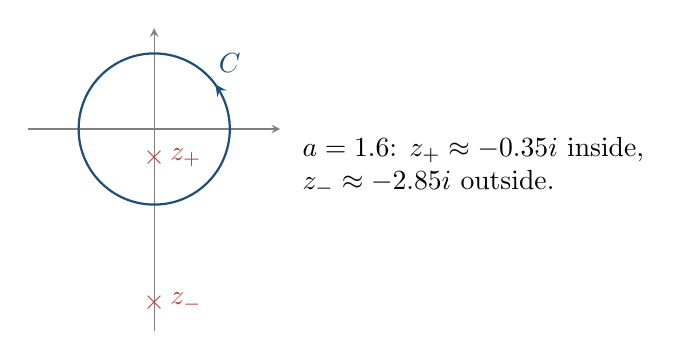
\begin{tikzpicture}[scale=0.8,>=stealth]
 \draw[gray,->] (-2,0)--(2,0);
 \draw[gray,->] (0,-3.2)--(0,1.6);
 \draw[courseblue,thick,postaction={decorate},decoration={markings,
  mark=at position 0.1 with {\arrow{>}}}] (1.2,0) arc(0:360:1.2);
 \node[exerciseframe] at (0,-0.45) {$\times$};
 \node[exerciseframe,right] at (0.1,-0.45) {$z_+$};
 \node[exerciseframe] at (0,-2.75) {$\times$};
 \node[exerciseframe,right] at (0.1,-2.75) {$z_-$};
 \node[courseblue] at (1.2,1.05) {$C$};
 \node[right,align=left] at (2.2,-0.6)
 {$a=1.6$: $z_+\approx-0.35i$ inside,\\ $z_-\approx-2.85i$ outside.};
\end{tikzpicture}
\end{lecturefigure}

\begin{exercise}
Evaluate the trigonometric integral
$\displaystyle\int_0^{2\pi}\frac{\cos^2\theta-\sin^2\theta+\cos\theta\sin\theta}{3-\sin\theta}\,d\theta$
from the beginning of this section.
\end{exercise}

\section{Improper integrals over the real line}
% Handwritten Lecture 23, pages 7--8. The handwritten notes split
% [-R,R] into [-R,0] and [0,R]; here they are combined. The example on
% page 8 is completed here.
We next compute integrals
\[
 \int_{-\infty}^{\infty}f(x)\,dx=\lim_{R\to\infty}\int_{-R}^{R}f(x)\,dx,
\]
where $f(x)$ is the restriction to $\R$ of a function $f(z)$ that is
holomorphic on a half-plane $\{\Imag z>-\epsilon\}$ except for finitely
many poles, none of which lie on the real axis. (This holds, for
example, for a rational function with no real poles.)

Let $H=\{z:\Imag z>0\}$ be the upper half-plane. For $R>0$ let $\gamma_R$
be the closed curve consisting of the segment $[-R,R]$ followed by the
semicircle $C_R(t)=Re^{it}$, $0\leq t\leq\pi$.

\begin{lecturefigure}
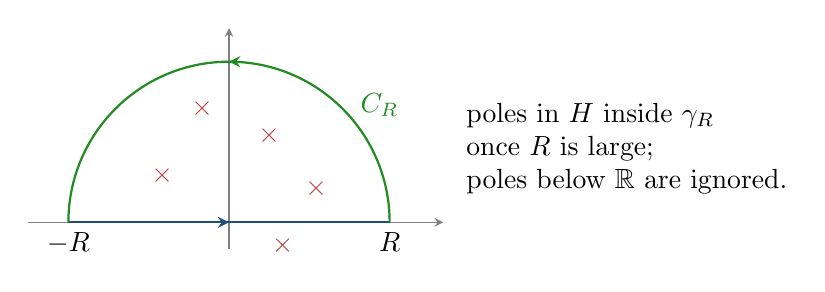
\begin{tikzpicture}[scale=0.85,>=stealth]
 \draw[gray,->] (-3,0)--(3.2,0);
 \draw[gray,->] (0,-0.4)--(0,2.9);
 \draw[courseblue,thick,postaction={decorate},decoration={markings,
  mark=at position 0.5 with {\arrow{>}}}] (-2.4,0)--(2.4,0);
 \draw[ForestGreen,thick,postaction={decorate},decoration={markings,
  mark=at position 0.5 with {\arrow{>}}}] (2.4,0) arc(0:180:2.4);
 \foreach \p in {(-1,0.7),(0.6,1.3),(1.3,0.5),(-0.4,1.7)}
  \node[exerciseframe] at \p {$\times$};
 \node[exerciseframe] at (0.8,-0.35) {$\times$};
 \node[below] at (-2.4,0) {$-R$};
 \node[below] at (2.4,0) {$R$};
 \node[ForestGreen] at (2.25,1.75) {$C_R$};
 \node[right,align=left] at (3.4,1.1)
 {poles in $H$ inside $\gamma_R$\\ once $R$ is large;\\ poles below $\R$ are ignored.};
\end{tikzpicture}
\end{lecturefigure}

The half-plane $\{\Imag z>-\epsilon\}$ is convex, hence simply connected.
Once $R$ exceeds the moduli of all poles $z_j$ in $H$, each such pole has
$w(\gamma_R,z_j)=1$, while any pole below the real axis lies outside
$\gamma_R$ and has winding number $0$. The residue theorem gives
\[
 \int_{-R}^{R}f(x)\,dx+\int_{C_R}f(z)\,dz
 =\int_{\gamma_R}f
 =2\pi i\sum_{z_j\in H}\operatorname{Res}_{z_j}(f).
\]
It remains to show that the semicircle contributes nothing in the limit.

\begin{theorem}\label{thm:improper}
Let $f$ be as above, and suppose there are $B>0$ and $R_0>0$ with
\[
 |f(z)|\leq\frac{B}{|z|^2}\qquad(\Imag z\geq0,\ |z|\geq R_0).
\]
Then
\[
 \boxed{\displaystyle\int_{-\infty}^{\infty}f(x)\,dx
 =2\pi i\sum_{z_j\in H}\operatorname{Res}_{z_j}(f),}
\]
the sum being over the poles of $f$ in the upper half-plane.
\end{theorem}
\begin{proof}
The bound shows $\int_{-\infty}^\infty|f(x)|\,dx<\infty$, so the improper
integral exists and equals $\lim_{R\to\infty}\int_{-R}^Rf$. For
$R\geq R_0$, the estimation lemma gives
\[
 \left|\int_{C_R}f\right|
 \leq\operatorname{Length}(C_R)\,\|f\|_{C_R}
 \leq\pi R\cdot\frac{B}{R^2}=\frac{\pi B}{R}\longrightarrow0.
\]
Letting $R\to\infty$ in the identity above gives the result.
\end{proof}

\begin{remark}
The same argument works if $|f(z)|\leq B/|z|^{1+a}$ for some $a>0$: the
semicircle integral is then at most $\pi B/R^a$.
\end{remark}

\begin{example}
We compute $\displaystyle\int_{-\infty}^{\infty}\frac{dx}{x^4+1}$, using
$f(z)=1/(z^4+1)$. For $|z|\geq2$ we have $|z^4+1|\geq|z|^4-1\geq|z|^4/2$,
so $|f(z)|\leq2/|z|^4\leq1/(2|z|^2)$ and Theorem~\ref{thm:improper} applies.
The poles are the fourth roots of $-1$, namely $e^{i\pi/4}$,
$e^{3i\pi/4}$, $e^{5i\pi/4}$, $e^{7i\pi/4}$; the first two lie in $H$.
At each pole $z_0$, Proposition~\ref{prop:res-simple-zero} gives
\[
 \operatorname{Res}_{z_0}f=\frac{1}{4z_0^3}=\frac{z_0}{4z_0^4}=-\frac{z_0}{4}.
\]
Since $e^{i\pi/4}+e^{3i\pi/4}=i\sqrt2$,
\[
 \boxed{\int_{-\infty}^{\infty}\frac{dx}{x^4+1}
 =2\pi i\cdot\Bigl(-\frac{i\sqrt2}{4}\Bigr)=\frac{\pi}{\sqrt2}.}
\]
\end{example}

\begin{exercise}
Use Theorem~\ref{thm:improper} to show that
$\displaystyle\int_{-\infty}^{\infty}\frac{dx}{(x^2+1)^2}=\frac{\pi}{2}$.
\end{exercise}

\end{document}
